%%%%%%%%%%%%%%%%%%%%%%%%%%%%%%%%%%%%%%%%%
% Imperial (EEE/EIE) Final Year Project Report Template 
% LaTeX Template
% Version 1.0 (28/06/16)
% Version 1.1 (20/01/28) 
% Version 1.2 (02/06/19)
% Modified by Aufar Laksana into a Final Year Project Report template
% For academic use only
%%%%%%%%%%%%%%%%%%%%%%%%%%%%%%%%%%%%%%%%%
%----------------------------------------------------------------------------------------
%	PACKAGES AND OTHER DOCUMENT CONFIGURATIONS
%----------------------------------------------------------------------------------------

\documentclass[12pt,a4paper]{report}
\usepackage[english]{babel}
\usepackage[utf8x]{inputenc}
\usepackage{amsmath}
\usepackage{amsfonts}
\usepackage{graphicx}
\usepackage{fancyhdr}
\usepackage[colorinlistoftodos]{todonotes}
\usepackage[toc,page]{appendix}
\usepackage{listings}
\usepackage[page]{totalcount}
\usepackage{color}
\usepackage{geometry}
\usepackage{caption}
\usepackage{subcaption}
\usepackage{float}
\usepackage[bottom]{footmisc}
\usepackage{diagbox}
\usepackage{gensymb}
\usepackage{mathpazo}

\usepackage{wrapfig}
\usepackage{lscape}
\usepackage{rotating}
\usepackage{epstopdf}


\usepackage{natbib} 



\definecolor{mygreen}{rgb}{0,0.6,0}
\definecolor{mygray}{rgb}{0.5,0.5,0.5}
\definecolor{mymauve}{rgb}{0.58,0,0.82}
\definecolor{mylilas}{RGB}{170,55,241}

\pagestyle{fancy}
\fancyhf{}
\lhead{Final Year Project}
\rhead{Final Report}
\rfoot{\thepage\ / \totalpages}

% \geometry{headheight=15pt}
% \geometry{footskip=0.4in}
% \geometry{textheight=694pt}
% \geometry{textwidth=400pt}



\lstset{ %
	basicstyle=\small,
	backgroundcolor=\color{white},   % choose the background color; you must add \usepackage{color} or \usepackage{xcolor}; should come as last argument
	breaklines=true,                 % sets automatic line breaking
	captionpos=b,                    % sets the caption-position to bottom
	commentstyle=\color{mygreen}\ttfamily\small,    % comment style
	escapeinside={\%*}{*)},          % if you want to add LaTeX within your code
	extendedchars=true,              % lets you use non-ASCII characters; for 8-bits encodings only, does not work with UTF-8
	frame=shadowbox,	                   % adds a frame around the code
	rulesepcolor=\color{teal},
	keepspaces=true,                 % keeps spaces in text, useful for keeping indentation of code (possibly needs columns=flexible)
	keywordstyle=\color{blue},       % keyword style
	language=C,                 % the language of the code
	morekeywords={*,...},            % if you want to add more keywords to the set
	numbers=left,                    % where to put the line-numbers; possible values are (none, left, right)
	rulecolor=\color{black},         % if not set, the frame-color may be changed on line-breaks within not-black text (e.g. comments (green here))
	showspaces=false,                % show spaces everywhere adding particular underscores; it overrides 'showstringspaces'
	showstringspaces=false,          % underline spaces within strings only
	showtabs=false,                  % show tabs within strings adding particular underscores
	stringstyle=\color{mymauve},     % string literal style
	tabsize=2,	                   % sets default tabsize to 2 spaces
}
\lstdefinelanguage{Mymatlab}{
	language=Matlab,%
	%basicstyle=\color{red},
	basicstyle=\ttfamily\footnotesize,
	breaklines=true,%
	morekeywords={matlab2tikz},
	keywordstyle=\color{blue},%
	morekeywords=[2]{1}, keywordstyle=[2]{\color{black}},
	identifierstyle=\color{black},%
	stringstyle=\color{mylilas},
	commentstyle=\color{mygreen},%
	showstringspaces=false,%without this there will be a symbol in the places where there is a space
	numbers=left,%
	numberstyle={\tiny \color{black}},% size of the numbers
	numbersep=9pt, % this defines how far the numbers are from the text
	emph=[1]{for,end,break},emphstyle=[1]\color{red}, %some words to emphasise
	%emph=[2]{word1,word2}, emphstyle=[2]{style},    
}
\lstdefinelanguage{TI}{
	sensitive = true,
	keywords={MVC,MVK,MVKLH,LDDW,LDW,NOP,STW,ZERO,LDDW,MPYDP,ADDDP,SUB,B},
	otherkeywords={% Operators
		>, <, ==
	},
	keywords = [2]{_circ_FIR_DP,loop,lend},
	keywordstyle=\color{blue},
	keywordstyle=[2]\color{purple},% for example
	numbers=left,
	numberstyle=\scriptsize,
	stepnumber=1,
	numbersep=8pt,
	showstringspaces=false,
	breaklines=true,
	frame=shadowbox,	                   % adds a frame around the code
	rulesepcolor=\color{teal},
	comment=[l]{;},
	morecomment=[s]{/*}{*/},
	commentstyle=\color{mygreen}\ttfamily\small,
	stringstyle=\color{red}\ttfamily,
	morestring=[b]',
	morestring=[b]"
}


\begin{document}

% Title Page
%\begin{titlepage}
%	% \newgeometry{top=25mm,bottom=25mm,left=38mm,right=32mm}
%	\setlength{\parindent}{0pt}
%	\setlength{\parskip}{0pt}
%	% \fontfamily{phv}\selectfont
%	
%	{
%		\Large
%		\raggedright
%		Imperial College London\\[17pt]
%		Department of Electrical and Electronic Engineering\\[17pt]
%		Final Year Project Report 2019\\[17pt]
%		
%	}
%	
%	\rule{\columnwidth}{3pt}
%	\vfill
%	\centering
%	
\includegraphics[width=0.7\columnwidth,height=80mm,keepaspectratio]{img/crest.png}
%	\vfill
%	\setlength{\tabcolsep}{0pt}
%	
%	\begin{tabular}{p{40mm}p{\dimexpr\columnwidth-40mm}}
%		Project Title: & \textbf{Augmented Reality-assisted Human Robot Interaction} \\[12pt]
%		Student: & \textbf{Aufar P. Laksana} \\[12pt]
%		CID: & \textbf{01093575} \\[12pt]
%		Course: & \textbf{EIE4} \\[12pt]
%		Project Supervisor: & \textbf{Professor Yiannis Demiris} \\[12pt]
%		Second Marker: & \textbf{Dr Tae-Kyun Kim} \\
%	\end{tabular}
%\end{titlepage}

\begin{titlepage}

% Defines a new command for the horizontal lines, change thickness here

%----------------------------------------------------------------------------------------
%	LOGO SECTION
%----------------------------------------------------------------------------------------


\includegraphics[width=8cm]{img/logo.png}\\[1cm] % Include a department/university logo - this will require the graphicx package
 
%----------------------------------------------------------------------------------------

\center % Center everything on the page

%----------------------------------------------------------------------------------------
%	HEADING SECTIONS
%----------------------------------------------------------------------------------------
\quad\\[1.5cm]
%\textsc{\LARGE MSc Thesis}\\[1.5cm] % Name of your university/college
\textsc{\Large Imperial College London}\\[0.5cm] % Major heading such as course name
\textsc{\large Department of Electrical and Electronic Engineering}\\[0.5cm] % Minor heading such as course title

%----------------------------------------------------------------------------------------
%	TITLE SECTION
%----------------------------------------------------------------------------------------
\makeatletter
\HRule \\[0.4cm]
{ \huge \bfseries Augmented Reality-assisted Human Robot Interaction}\\[0.4cm] % Title of your document
\HRule \\[1.5cm]
 
%----------------------------------------------------------------------------------------
%	AUTHOR SECTION
%----------------------------------------------------------------------------------------

\begin{minipage}{0.4\textwidth}
\begin{flushleft} \large
\emph{Student:}\\
Aufar P. Laksana% Your name
\\[1.2em]
\emph{CID:}\\
01093575
\end{flushleft}
\end{minipage}
~
\begin{minipage}{0.4\textwidth}
\begin{flushright} \large
\emph{Project Supervisor:} \\
Professor Yiannis Demiris
% Uncomment the following lines if there's a co-supervisor
\\[1.2em] % Supervisor's Name
\emph{Second Marker:} \\
Dr. Tae-Kyun Kim % second marker's name
\end{flushright}
\end{minipage}\\[3cm]
\makeatother


%----------------------------------------------------------------------------------------
%	DATE SECTION
%----------------------------------------------------------------------------------------

{\large Final Year Project Report 2019}\\[0.5cm]
{\large \emph{MEng Electronic and Information Engineering}}\\[0.5cm]
{\large \today}\\[2cm] % Date, change the \today to a set date if you want to be precise

\vfill % Fill the rest of the page with whitespace

\end{titlepage}

\addvspace{6em}

\renewcommand{\abstractname}{\LARGE Abstract}

\addcontentsline{toc}{chapter}{Abstract}

\begin{abstract}

Text of the Abstract.

\end{abstract}

\tableofcontents

\newpage

\chapter{Introduction and Requirements}

\section{Introduction}
This report was written as part of the Final Year Project for the MEng Electronic \& Information Engineering course. The project was supervised by Dr. Yiannis Demiris at the Imperial College London.

\section{Motivation}

\chapter{Background}
This project is focused on computer vision for detecting and tracking humans in the surroundings, estimating their trajectories and distance from the PWU, the reactive control systems that prevent collisions with the detected objects as well as the augmented reality display to provide visual cues to the PWU.

\section{Human Detection}
Human detection is a subset of the classic computer vision problem of object detection. In order to develop an augmented reality system that will help PWUs to navigate in public spaces, it is essential for the system to be able to discern humans from the surroundings.

\subsection{Direction of Research}
 The problem arises in crowded areas, whereby individuals are occluded by other people or objects in front of them, leaving only certain body parts visible. As such, we began our research with the problem of being able to detect people in images where identifiying parts of the body are not always visible.

\subsection{Review of Existing Methodologies}
A related field of research is that of people counting and human detection in visual surveillance in public areas. Where the problem differs is that surveillance benefits from being able to rely on cameras with a good view of the crowd from above, whereas for a PWU, the camera will not have as high of a vantage point, making detecting every single individual in a crowd impossible. 

\paragraph{} Despite the disadvantage, similar techniques can be used to detect humans in video. Most methods can be classified into two categories \cite{Hou2010}. The first technique, foreground detection, attempts to model the background of an image and then detect the changes that occur between frames. The second category involves exhaustively searching the image with a scanning window, and deciding if each window can be classified into a human shape.

\begin{figure}[ht]
	\begin{subfigure}[b]{.5\textwidth}
		\centering
		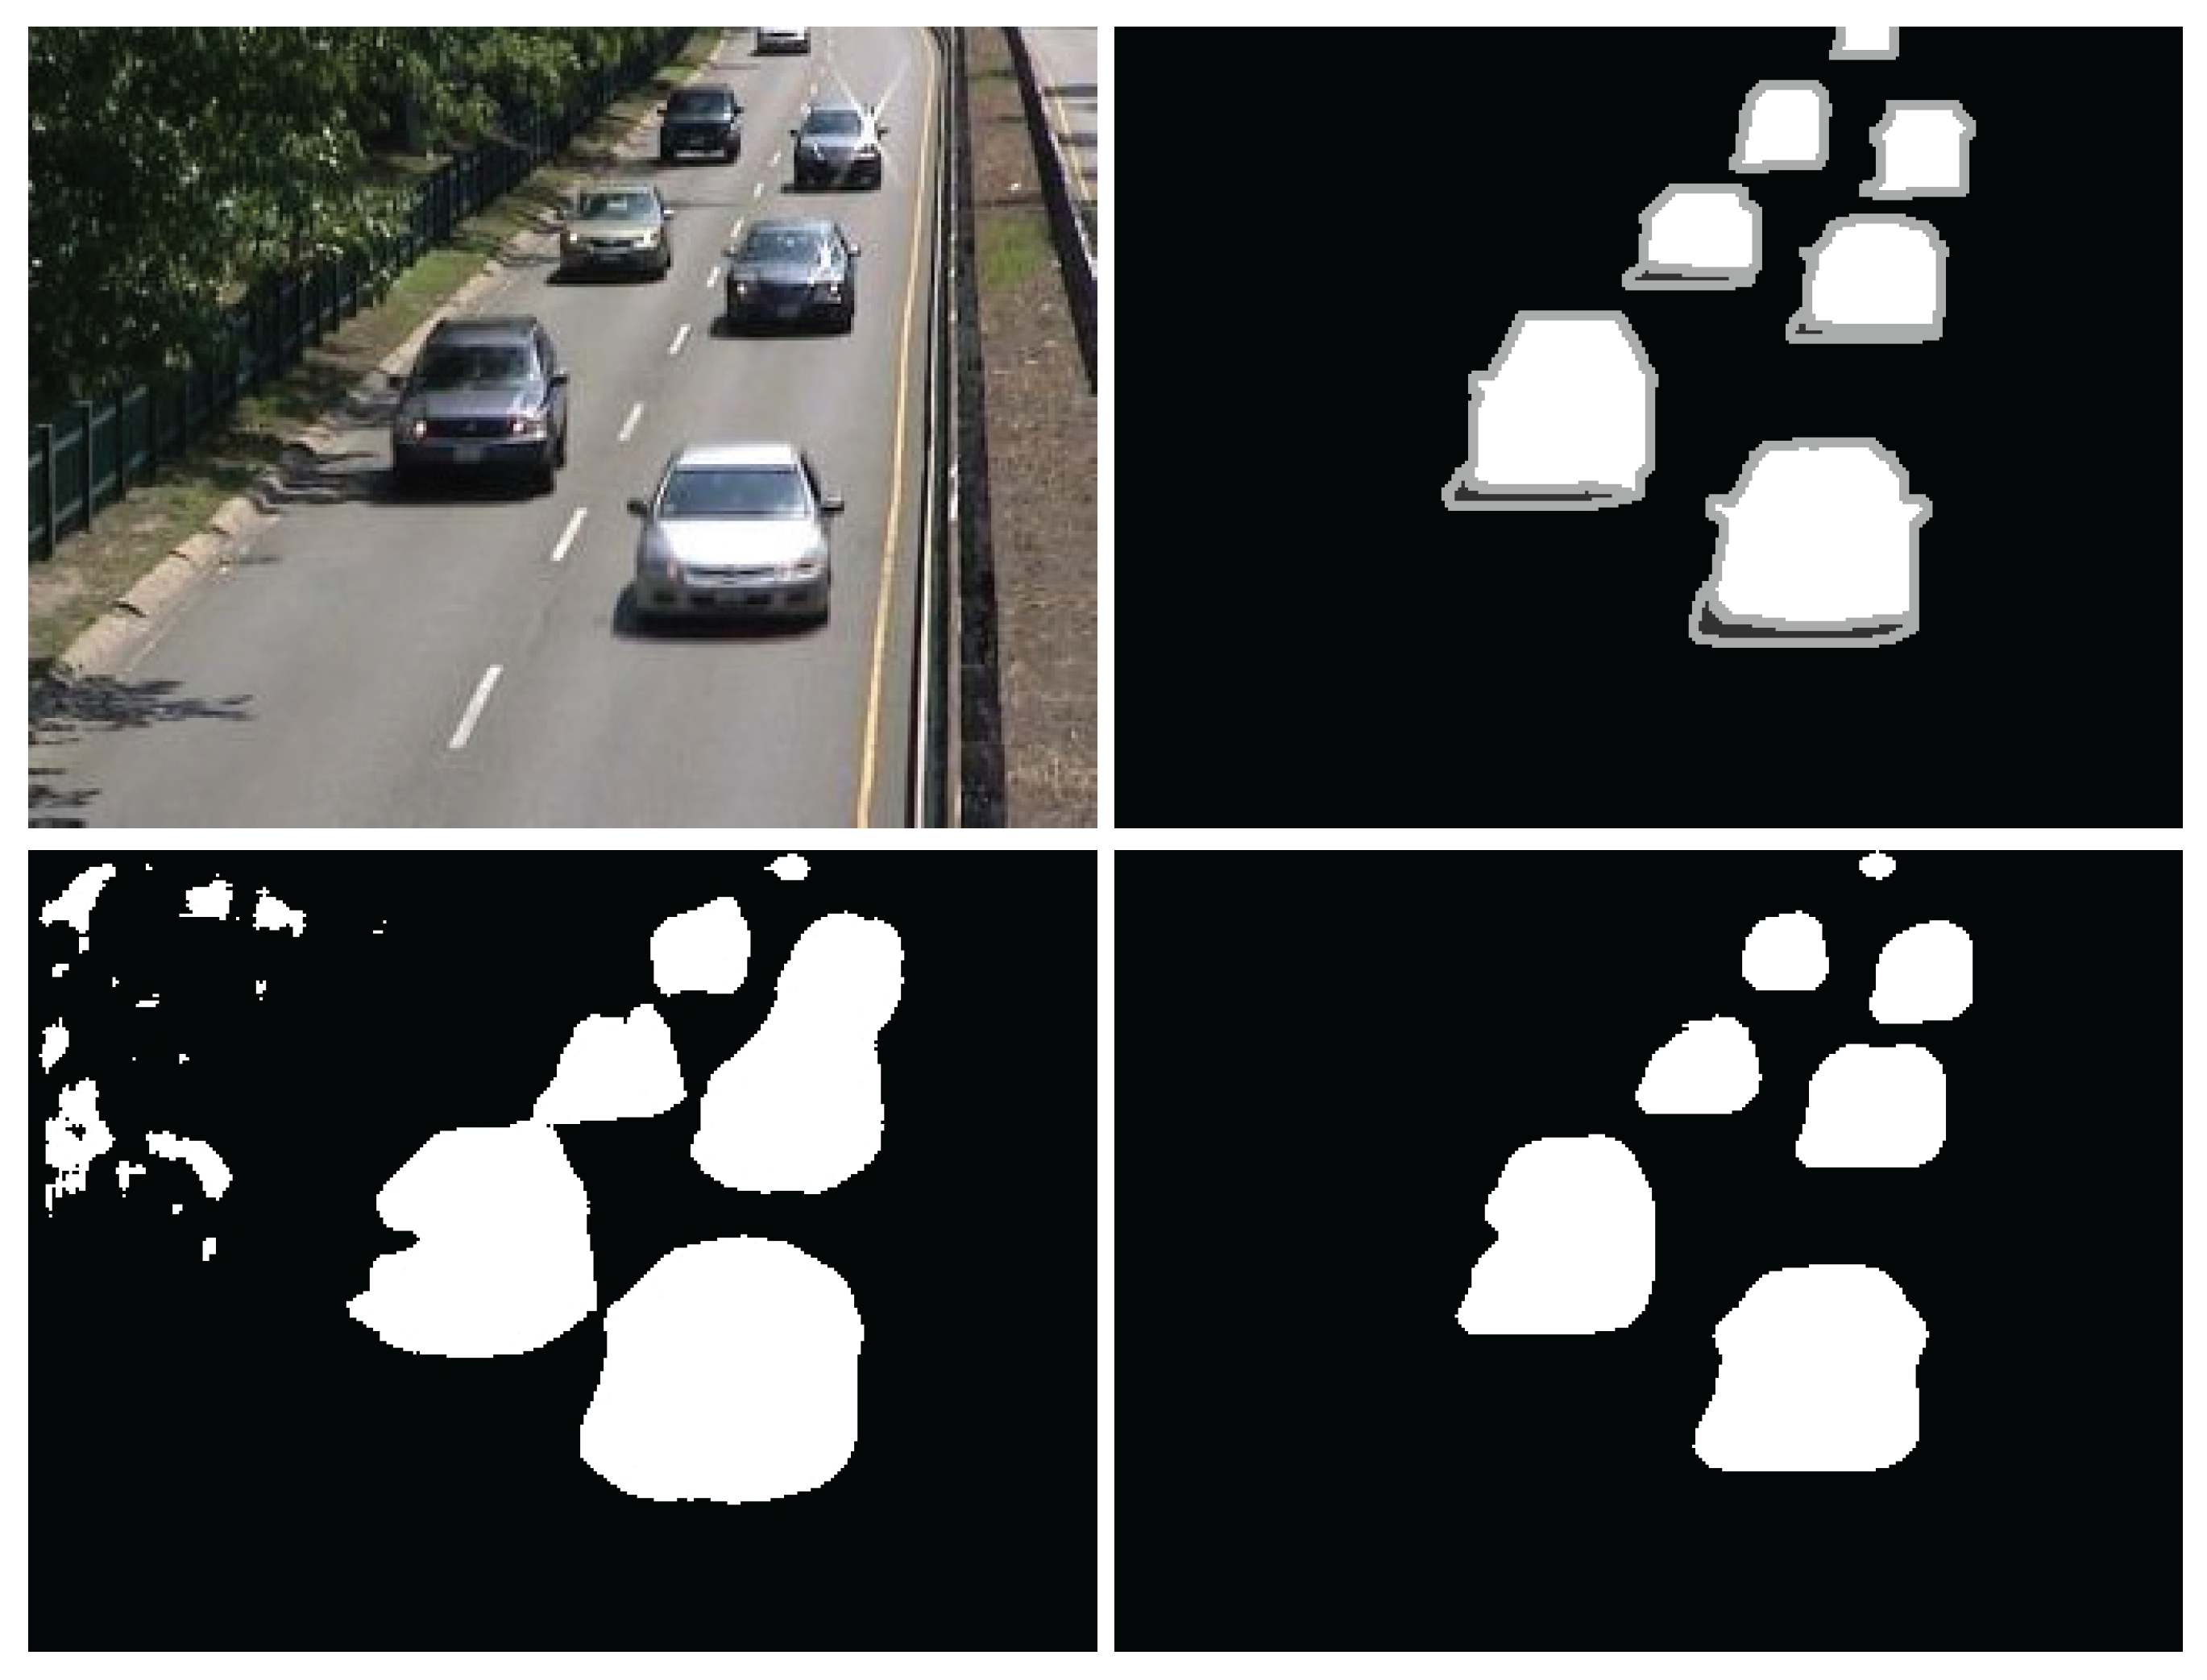
\includegraphics[width=.9\linewidth]{img/chapter2_background/robustBackgroundSubtraction.png}
		\caption{Foreground Detection \cite{Zeng2017}}
	\end{subfigure}%
	\hspace{\fill} 
	\begin{subfigure}[b]{.5\textwidth}
		\centering
		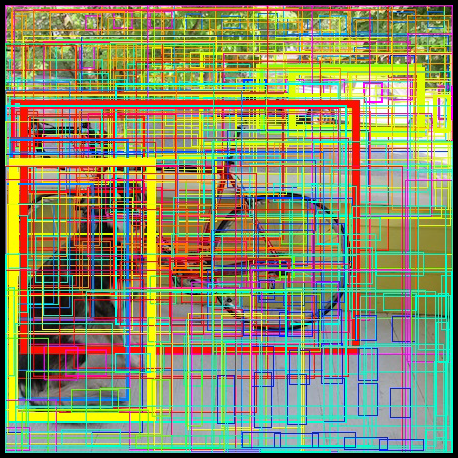
\includegraphics[width=.675\linewidth]{img/chapter2_background/yoloBBBoxes.png}
		\caption{Scanning Window \cite{Redmon}}
	\end{subfigure}
	\vspace{-2\baselineskip}
	\begin{center}
		
		\caption{Comparison of Foreground Detection and Scanning Windows}
		\label{fig:foregroundVsScanning}
	\end{center}
	\vspace{-2\baselineskip}
\end{figure}

\subsubsection{Foreground Detection}
Background subtraction is a widely used approach for detecting moving objects \cite{Piccardi2004}. A temporal average filter can be used to find the median of all the pixels in an image to form a reference image. Frames with moving objects can then be compared pixelwise to the reference, and a threshold set to determines if the pixel is part of the background or foreground. People counting and human detection can then be achieved by segmenting the foreground image into individuals.

\paragraph{} However, this technique often relies on a static camera in a well placed location. This brings up several reasons as to why this method would not be suitable for this project. Firstly, the camera available is part of a head-mounted augmented reality device. The wearer has the ability to move the camera in 6 degrees of freedom. Secondly, the wearer will also be navigating a powered wheelchair. As a result, the background is constantly changing, and the reference image would require constant recomputation before human detection can even begin.

\subsubsection{Scanning Windows}
Due to the ever-changing surroundings of a mobile robot, a better approach for object detection is to exhaustively search an image using scanning windows and determining if an object was detected in each window. However, it must be noted that this method is computationally expensive. In order to achieve real-time detection on a mobile robot, the use of a graphics processing unit (GPU) should be considered \cite{Hirabayashi}.

\subsubsection{Classical Object Detection}

\paragraph{Haar Cascades}
Haar cascades classifies images based on the value of simple features \cite{Viola2001}, which are variants of the difference between the sum of pixel values in rectangular regions. An intermediate representation of the original image is used to rapidly compute a small set of representative rectangular features.

\paragraph{}A cascade of classifiers is then used to determine if the region is detected as a human. The detection process is that of a degenerate decision tree, where a positive result in the first cascade will trigerr an evaluation in the second, more successful classifier. As such, the initial classifier can eliminate a large number of negative examples with very little processing. After several stages, the number of sub-windows has been reduced radically

\paragraph{Histograms of Oriented Gradients}
The method proposed is implemented by dividing the image window into small spatial regions and calculating a local 1-D histogram of gradient directions for all the pixels in the region. The combined local histograms form the overall feature representation of the image.

\paragraph{}The detection window is tiled with the Histogram of Oriented Gradient (HOG) descriptors. In the original paper \cite{Dalal2005}, these feature vectors were then used in a conventional SVM based window classifier  to give human detections.

\subsubsection{Deep Learning Object Detection}
Modern approaches for human detection largely depend on Deep Convolutional Neural Networks (CNN). The approach provides the best in class performance, as well as scaling effectively with more data. An added advantage of using CNN based object detection systems for this project is that they are also capable of detecting multiple classes of objects.

\paragraph{}An issue with CNN approaches is that the methods are trying to draw bounding boxes around objects of interest in images. However, we do not know the number of objects in the image beforehand. As such, to be completely sure every object has been detected, a naive solution is to take a huge number of regions and attempt to classify all the objects in the region, a computationaly expensive process.

\begin{figure}[ht]
	\centering
	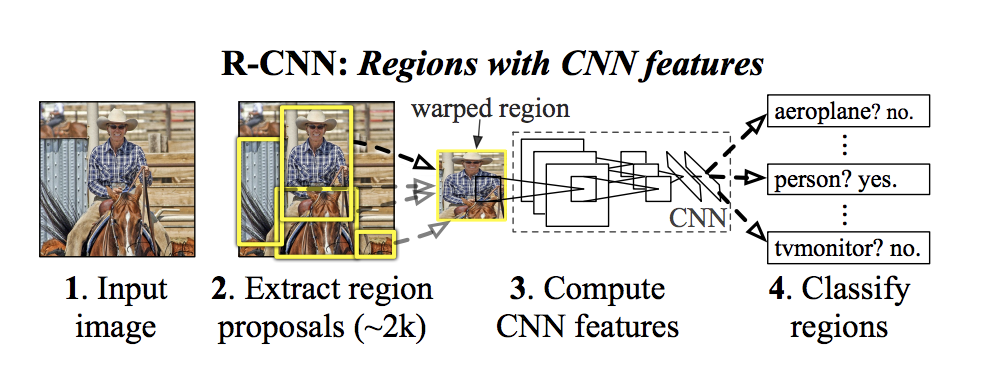
\includegraphics[width=.9\linewidth]{img/chapter2_background/rcnn.png}
	\caption{R-CNN Approach}
\end{figure}

\paragraph{R-CNN} The R-CNN method uses a selective search to extract 2000 regions from an image \cite{Girshick2014}. The regions are selected by generating a large number of candidate regions and using a greedy algorithm to recursively combine similar regions into larger ones. The regions are then fed into a CNN that acts as a feature extractor and the output dense layer consists of the features extracted from the image, which are then fed into an SVM to classify the presence of objects in the region.

\paragraph{}The major disadvantage to this approach is the amount of time required to train the network. Each training image has to be classied once for each of the 2000 region proposals. Furthermore, the selective search algorithm is a fixed algorithm (no learning is done), and as such, could lead to generation of bad candidate region proposals.

\paragraph{YOLO} Whereas R-CNN uses regions to localize the object within an image, You Only Look Once (YOLO) looks at the image as a whole and uses a single CNN to predict the bounding box and the class probabilities \cite{Redmon}. By looking at the image as a whole, the network can use features from the entire image to predict each bounding box.

\begin{figure}[ht]
	\centering
	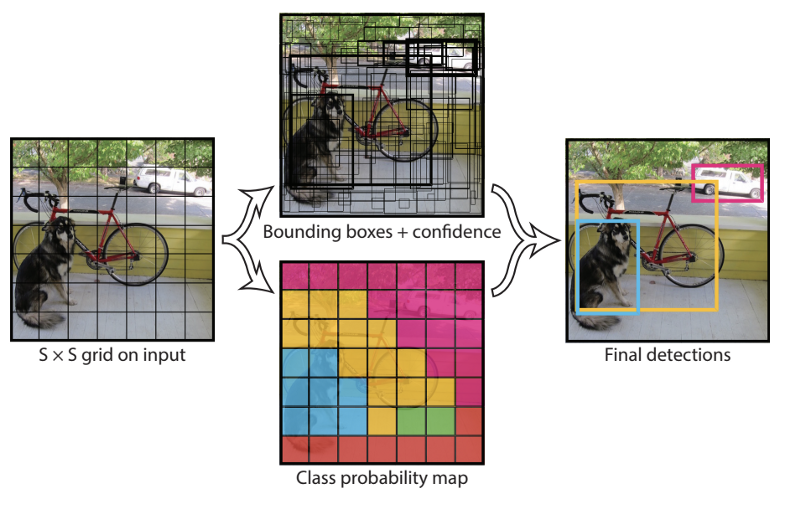
\includegraphics[width=.6\linewidth]{img/chapter2_background/yoloApproach.png}
	\caption{YOLO Approach}
\end{figure}

The model divides the image into an $S \times S$ grid, and for each cell, predicts a number of bounding boxes, the confidence for those boxes and the class probabilities.

\subsection{Comments} \label{sec:detector}
As seen from the research, we can clearly see that there are many ways to solve the human detection problem. The classical approaches, although computationally efficient, are siginficiantly outperformed by the deep learning approaches. For a mobile robot in a public area, we want to be able to detect almost all humans in the surroundings to better inform the PWU.

\paragraph{}However, the major disadvantage of the deep learning approach is the time taken to train the network, as well as the requirement of a GPU to achieve real-time performance. These issues will be addressed in a later section of the report.

\section{Object Tracking}
Object tracking can be defined as the ability to detect objects in consecutive frames and determining if the same objects are present. The techniques are often used in security and surveillance to track individuals across multiple cameras. A more relevant use of object tracking is in augmented reality with ARMarkers to allow for more accurate placements of holograms as the user moves through the AR world.

\subsection{Direction of Research}
 A common scenario for PWU in public spaces is having multiple people walking in the surroundings. Ideally, the augmented reality system should be able to track the same people across frames to be able to determine their direction of motion. As such, we focus our research on the multiple object tracking (MOT) problem in real-time. For an augmented reality system for a PWU, the object tracking must be done in real-time in order to feedback to the PWU. This narrows our field of research to online object tracking techniques.
 
\subsection{Review of Exisiting Methodologies} \label{sec:objectTrack}
 Pedestrian detection is often achieved by using a high quality object detector and associating the detections across frames \cite{Dicle2013}. The associations are based on the appearance and location similarity. Furthermore, it is possible to discern simple motion patterns from the tracked pedestrians, allowing for more accurate tracking.
 
\subsubsection{SORT}
\paragraph{Methodology} The Simple Online and Realtime Tracking (SORT) method relies on the accurate detections of a CNN to calculate bounding boxes of the tracked objects across frames \cite{Bewley2016}. The technique estimates the inter-frame displacements of each detected objects with a linear constant velocity model. The state of each tracked object is modelled using the bounding box centroids $u$ and $v$, the scale and aspect ratio, $s$ and $r$.

\[x = [u, v, s, r, \dot{u}, \dot{v}, \dot{s}] \]

When a new detection is associated with a tracked object, the bounding box of the new detection is used to update the tracked object state, and using a Kalman filter to update the velocity components \cite{Kalman1961}. To determine associations between new detections and tracked targets, the SORT algorithm relies on the intersection-over-union (IOU) distance between each detection and the predicted bounding boxes of all the existing targets.

\paragraph{} For every detection to be tracked, a uniqe tracker identity must be created and destroyed when the object enters and leaves the image. The original implmentation of the algorithm relied on a $IOU_{min}$ value to signify the existence of an untracked object. The tracks are then terminated if they are not detected for an allotted number of frames, to prevent the unbounded growth of trackers.

\paragraph{Limitations}
Due to the simplicity of the association metric, the significant overhead and complexity of object re-identification is removed, allowing for the system to work in real-time applications. However, this also reduces the accuracy of the tracking, since occlusions will spawn new trackers for the same objects. Furthermore, the accuracy of the tracking is largely dependent on the object detector providing accurate bounding boxes.

\subsubsection{Deep SORT}
The original SORT suffered from a high number of identity switches, since the association metric was only accurate if the state estimation uncertainty was low. Wokje proposed a solution to the issue by learning a deep association metric on a re-identification dataset \cite{Wojke2018}. 

\paragraph{Methodology} The tracking and Kalman filtering in Deep SORT is mostly identical to the original SORT implementation. However, Deep SORT uses a Mahalonibis distance as an association metric between the Kalman predicted states and new detections. It further uses a second metric, whereby an appearance descriptor is calculated for each bounding box. A gallery of the previous $L_{k} = 100$ descriptors are kept for each track. The algorithm then iterates and measures the smallest cosine distance between the existing tracks and the detection.

\paragraph{} The appearance descriptor is implemented using a CNN that has been trained offline on a person re-identification dataset. The Github implementation of the Deep SORT algorithm uses a simple nearest neighbour query without any additional metric learning.

\paragraph{Limitations}
Although the accuracy of the the tracking is improved and the issue of occlusions is reduced, the increased complexity of the algorithm requires more computational power. As stated in the paper, a modern GPU would be required to run this in real-time, due to the need for an appearance descriptor to be calculated for each detection.

\subsection{Comments} \label{sec:objectTrackComments}
For this project, we have limited ourselves to researching simple object tracking methods that work in real-time. We can clearly see a trade-off between accuracy of tracking and computational power. Further investigation into the hardware available and the importance of object tracker accuracy will be needed to decide what method would be best for the augmented reality system.

\section{Head and Body Pose Estimation}
Pose estimation is a general computer vision problem where we attempt to detect the position and orientation of an object. This process can be achieved by detecting keypoint locations that describe the pose of the object. For instance, in body pose estimation, we identify the joints in the body.

\subsection{Direction of Research}
An interesting concept to explore is that of head and body pose estimation as a way of infering the direction a person is walking in. For instance, people tend to look in the direction they are currently walking, but should they want to change direction, they also tend to look in that direction before changing \cite{Valenti2012}. Similarly, if we can determine the body pose of a person, the system will be able to tell if a person is walking to or away from the PWU without relying on depth sensors.

\subsection{Review of Existing Methodologies}

\subsubsection{Head Pose Estimation} \label{sec:backHeadPoseEstimation}
Head pose estimation is intrinsically linked with visual gaze estimation \cite{Murphy-Chutorian2009}. If we can characterize the direction and focus of a person's eyes, it may be possible to determine the direction they will walk in next.

\paragraph{Facial Landmark Detection}
Before head pose estimation can be done, keypoints on the face must be detected \cite{Kazemi2014}. These points will then be used to solve a Perspective-n-Point (PnP) problem to determine the head pose. There are many facial landmark detection techniques, depending on the number of landmarks to be detected. As the number of landmarks increase, the more accurate the pose estimation can be. However, it also increases the complexity of the detection, and as such, it becomes a trade-off between the two factors.

\subsubsection{Body Pose Estimation} \label{sec:backBodyPoseEstimation}
An idea we wish to explore is using the body pose of an individual to estimate the direction they are walking in. If the system can discern between a person's back or front, we can infer the motion, since people do not normally walk backwards. A limitation of our system is that it has to be done in real time for it to be effective. As such, the techniques we can explore are limited by the hardware available.

\paragraph{PoseNet} A common approach for body pose estimation is to employ a person detector and perform single-person pose estimation for each detection, known as a top-down approach. PoseNet is a real-time human pose estimator with a web-browser implementation that runs on Tensorflow.js, making it easily available to anyone. The implementation is based on the works of Papanderou and Zhu \cite{Papandreou2017} in building a network that utilizes the Faster-RCNN model as an object detector to obtain accurate bounding boxes of people in an image \cite{Ren2017}. The keypoints are then calculated using a a ResNet \cite{He2016} by predicting activation heatmaps and offsets.

\paragraph{OpenPose} Top-down approaches can be limited by the failure of the person detector. This is especially common when two individuals are very close to each other, and the detector is unable to differentiate between them. In contrast the bottom-up approach, which is based on partitioning and labeling an initial pool of body part candidates into subsets \cite{Pishchulin}, is able to deal with an unknown number of people, and can infer that number by linking the part hypotheses.

\begin{figure}[ht]
	\centering
	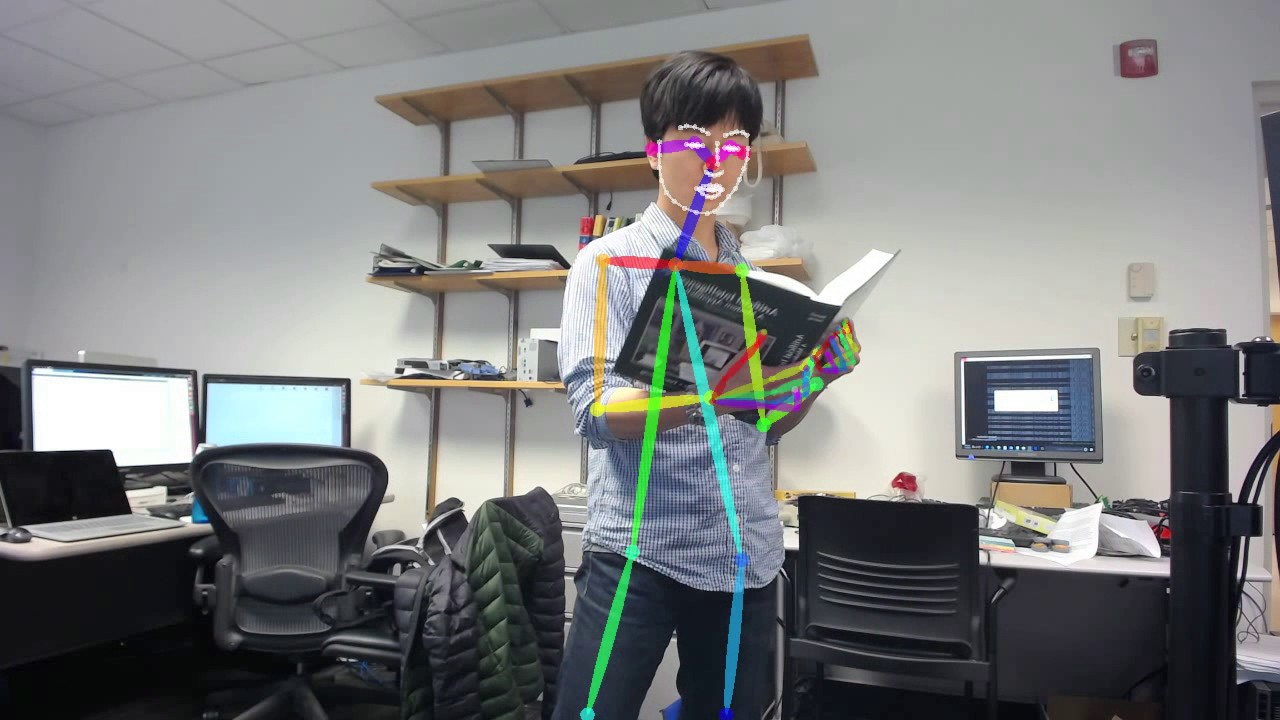
\includegraphics[width=.7\linewidth]{img/chapter2_background/openpose.jpg}
	\caption{OpenPose body pose detection \cite{Cao2017}}
\end{figure}

\paragraph{} As such, OpenPose presents a method of multi-person pose esimtation using a bottom-up approach \cite{Cao2017}. The method relies on \textit{partial affinity fields} (PAFs), a representation that encodes unstructured pairwise relationships between body parts. The network produces the 2D confidence maps of body part locations and PAFs, and through greedy inference, the network outputs the 2D keypoints for all people in the image.

\subsection{Comments}
Head and body pose estimation is a vast field of research, with dozens of effective real-time estimation methods. This project is not focused on achieving the best body/head pose estimation, but rather, in utilizing existing frameworks to infer directions of individuals. As such, we have refrained from delving too deep into the theory of body pose estimation, and instead, have attempted to choose a method from available implementations.

\section{SLAM}
The term mapping refers to a system that will create a map of the surrounding areas, by detecting objects such as walls and other obstacles. In order to help users navigate, the system must analyse the surroundings for potential dangers. As such, it is important to build up a thorough and complete map.

\paragraph{}A fundamental method for robot navigation is the Simultaneous Localization And Mapping (SLAM) method. The process allows the system to predict the trajectory of the robot and the location of all objects on-line, without the need of an \textit{a priori} knowledge of the robots location \citep{Bailey2006a}. The method estimates the pose of the robot relative to landmarks which are detected. The popularity of SLAM increased with the emergence of indoor applications of robotic devices.

\subsection{Direction of Research}
For a PWU to navigate a wheelchair effectively through public spaces, they need to be able to avoid colliding with people or obstacles. An accurate map of the surroundings is key to solving this issue. However, some techniques rely on pre-existing maps of the area. A PWU may navigate their wheelchair to new locations, and can not rely on pre-existing maps for accurate navigation. Rather, the goal is to build up a real-time map of the surroundings that is accurate enough to avoid collisions.

\subsection{Review of Existing Methodologies}
A review of SLAM techniques can be found in \cite{Cadena2016}, which also outlines the standard formulation of the SLAM problem as that of a Maximum a posteriori (MAP) estimation. The formulation relies on Bayes theorem, and using the prior knowledge of the robots pose to maximize the likelihood to estimate the current position of the robot. The variables required to estimate the position are the robot poses, the position of landmarks and the calibration parameters of the sensors.

\paragraph{}In order to build an accurate map of the surroundings, the calibration of the sensors providing the measurements is a crucial step. The choice of sensors also matter, as the type of data returned by the sensor may affect the computational complexity of the SLAM algorithm. As such, it is common to have a module in the system that deals with the extraction of relevant features from the sensor data.

\paragraph{}A fairly common assumption in SLAM approaches is that the world is static and remains unchanged as the robot moves. This becomes an issue with the goal of this project, which hopes to achieve the ability to detect human objects walking around the wheelchair. This issue will be addressed in a later section.

\subsubsection{Visual SLAM}
Visual SLAM (vSLAM) is an implementation of SLAM that relies on visual inputs only. As stated in \cite{Taketomi2017}, vSLAM is suitable for AR due to the low computational algorithms that can be implemented on the limited resources of an AR headset. The technique of vSlam is mainly composed of three modules:

\paragraph{Initialization}
In the initialization stage, camera pose estimation is conducted, to transform objects in a 2D image from the camera into a 3D co-ordinate system that the robot understands. This process determines the position and orientation of the camera relative to the object. A part of the environment is reconstructed as part of the initial map using the global co-ordinate system of the robot.

\paragraph{Tracking}
Here, the reconstructed map is used to estimate the pose of the camera with respect to the map. Feature mapping or feature tracking is conducted on the images in order to get a 2D-3D correspondence between the image and the map. The camera pose can then be calculated from the correspondences by solving the Perspective-n-Point problem \citep{Nister2004}. This allows the system to identify where on the map the robot currently is.

\paragraph{Mapping}
When the robot passes through an environment that has previously not been mapped, the 3D structure of the surroundings is calculated from the camera images. The structures are then added to the existing map of the environment.

\subsection{Comments}
Due to the freedom in movement of an augmented reality headset camera, a system that relies solely on visual inputs may not be able to detect all obstacles in the surroundings. For instance, a limitation is that the PWU will not be able to extend their head backwards to view objects behind them. As such, it becomes important to consider the sensors available on powered wheelchairs, and utilize them to build an accurate map of the surroundings.

\section{Augmented Reality Headsets}
The improvements in augmented reality technology has spurred research into the use of AR devices in everyday tasks. The availability of commercial devices has also encouraged developments in the field, with products such as the Microsoft Hololens and the Magic Leap One.

\subsection{Direction of Research}
The augmented reality system built for this project needs to be able to give visual prompts to the PWU. As such, a device that already has the ability to create holograms is key. Furthermore, most AR devices have built in cameras to perceive the world around the user. We hope to be able to access the cameras on the device to do object detection and tracking.

\subsection{Review of Existing Methods}

\subsubsection{Microsoft Hololens}
The Microsoft Hololens is an untethered holographic computer, allowing for the display of 3D holograms pinned to real world objects. The Hololens is equipped with an array of sensors, making it an ideal choice of hardware for this project.

\paragraph{Holograms}The Microsoft Hololens is able to blend real world and virtual content into environments where digital and physical objects can co-exist and interact. The term 'Mixed Reality' was first introduced by \cite{Milgram1994}, and refers to the blending of the physical and virtual worlds.

\paragraph{}The Hololens allows the developer to create 'Holograms', which are objects of light and sound that are displayed by the headset. Users are able to interact with the holograms through voice, gaze and gestures. Enhanced environment apps are applications that facilitate the placement of digital information on the user's current environment \citep{Microsofta}. An example of an enhanced environment application is placing markers in augmented reality on objects that the user can interact with in both the physical and digital worlds. 

\paragraph{Hardware Specifications} As part of our research, we highlight the sensors on the device that may be relevant to the project. A full hardware specification is available online \cite{Microsoft2015}. 

\begin{itemize}
	\item 1 Intertial Measurement Unit (IMU)
	\item 4 Environment understanding cameras
	\item 1 Depth Camera
	\item 1 2MP Photo/HD video camera
\end{itemize}

\paragraph{} Most importantly, the Hololens has a video camera. Preliminary research shows that it is possible to access the camera data directly, making it a suitable choice for the project.

\paragraph{Personal Robotics Lab} The use of augmented reality devices to help PWUs is a research topic actively pursued by members of the Personal Robotics Lab at Imperial College London. Previous work has explored the use of augmented reality as a visualization tool to help PWUs understand the system dynamics of the wheelchair they operate, displaying visual cues that indicate the direction of travel of assistive control \cite{Zolotas2018}. Other work involves using the camera to detect objects of interest in the environment, and developing a system that navigates the wheelchair to the detected objects through gaze and eye tracking \cite{Chacon-Quesada}.

\begin{figure}[ht]
	\centering
	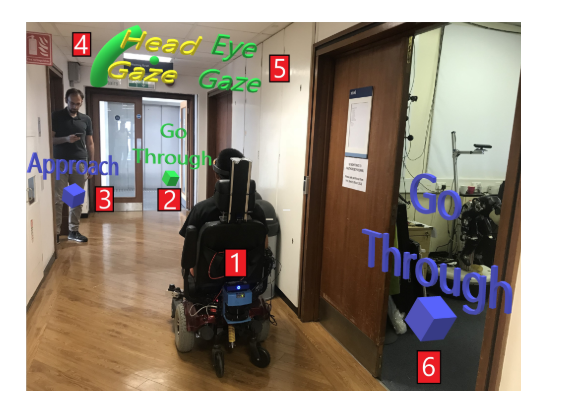
\includegraphics[width=.5\linewidth]{img/chapter2_background/AR_Interface.png}
	\caption{AR visualizations and markers for interaction \cite{Chacon-Quesada}}
\end{figure}

\subsection{Comments}
Although other AR-devices exist on the market, due to the availability of the Microsoft Hololens in the Personal Robotics Lab, as well as the research done by individuals, it is in the best interests of this project to use the Hololens as the main augmented reality device for this project.

\chapter{Requirements Capture}

\section{Project Deliverable}
The objective of this project is to develop an augmented reality system that can be used by powered wheelchair users (PWUs) to assist them in navigating their powered wheelchairs in public spaces with many people walking in the surroundings. The system should be able to detect the presence of individuals and infer their position relative to the PWU, and by extensions, estimate their direction of travel.

\paragraph{}We propose a system that uses the Microsoft Hololens augmented reality headset as the main input and visualization tool. The PWU would wear the headset as they operate the powered wheelchair, allowing the system to create visualizations of potential obstacles and collisions. Furthermore, the system would also encompasses the reactive control aspect of the powered wheelchair. Should an individual be detected as walking in the wheelchairs trajectory, the system will send control signals to the powered wheelchair to slow down or completely stop depending on how far the target is from the wheelchair.

\paragraph{} By definition of the requirements, we can divide the project into three parts: Human Detection and Direction, Obstacle Mapping \& Visualization, and finally Reactive Control.

\section{Human Detection and Direction}
The requirements of the Human Detection and Direction (HDD) system is to be able to use a video stream of the surroundings to determine the position and direction of people. The Hololens has a built in camera that can be used to take photos of the surroundings of the user \cite{Chacon-Quesada}. We will leverage this ability to create a video stream.

\paragraph{}The actual HDD system is implemented on another computer with access to a GPU. We utilize the GPU to be able to do real-time object detection and pose estimation of detected individuals. The system should be able to infer the direction individuals are walking in, as well as their real-world positions relative to the PWU.

\paragraph{Features} 
\begin{itemize}
	\item Creating a live video stream using camera.
	\item Streaming the live video to accompanying computer.
	\item Object detector trained on humans/pedestrians.
	\item Object tracker to track detected humans, and determine their direction.
	\item Body/Head pose estimator to determine direction of travel.
	\item Stream detections back to the Hololens for visualization.
\end{itemize}

\section{Obstacle Mapping \& Visualization }
This project utilizes the Microsoft Hololens as a visualization and spatial mapping tool. The HDD system will output its detections and directions to the Hololens, which is used to create visualizations that will help the PWU. Examples of the visualization include arrows that indicate direction of movement, as well as alerting the user to potential collisions.

\paragraph{Features}
\begin{itemize}
	\item Receiving detection/direction data from HDD system.
	\item Utilize Camera to World transforms of the Hololens Camera to get World co-ordinates of people.
	\item Create holographic visualizations to help PWU understand the direction people are walking in.
	\item Create a map of obstacles for Reactive Control.
\end{itemize}
 
\section{Reactive Control} \label{sec:reactive}
The powered wheelchair (ARTA) available in the Personal Robotics Lab (PRL) can be manually operated using a joystick. The goal of the project is for the PWU to be able to wear the Hololens as an aid for navigation in public spaces. As such, it would be beneficial for the PWU if the wheelchair had the ability to reactively control the device to prevent collisions with detected objects.

\paragraph{Features}
\begin{itemize}
	\item Receiving object detections in front of wheelchair.
	\item Prevent wheelchairs from driving into objects.
\end{itemize}


\bibliographystyle{unsrt}
\bibliography{fyp_report.bib}

\end{document}